\chapter{Data and Feature Engineering Architecture}
\label{ch:data_and_features}

\section{Data Pipeline and Sample Construction}
My empirical sample comprises daily stock prices, trading volumes, and quarterly financial accounting metrics for active and historical S\&P 500 constituent equities from December 31, 2014, through December 31, 2024. The active evaluation window spans January 1, 2015, to December 31, 2024, yielding 2,516 trading days and over 1.25 million stock-day observations \citep{gu2020empirical}.

Daily closing prices, dividend payments, stock splits, and trading volumes are ingested from Yahoo Finance and cross-verified against Bloomberg Terminal records. Daily risk-free rates ($R_{f,t}$) along with daily Fama-French 5-Factor returns ($Mkt-RF_t, SMB_t, HML_t, RMW_t, CMA_t$) and Carhart Momentum ($MOM_t$) are retrieved directly from the Ken French Data Library \citep{fama1993common, fama2015five, carhart1997on}.

\subsection{Point-in-Time Bloomberg Filing Date Alignment}
A common issue in empirical finance studies is lookahead bias caused by indexing corporate accounting metrics to fiscal period end-dates. In practice, financial statements for a fiscal quarter ending on December 31 ($t_{\text{fiscal}}$) are published weeks or months later during the 10-K or 10-Q SEC filing process \citep{lopez2018advances}.

To eliminate lookahead contamination, my data pipeline (\path{src/data_pipeline.py}) ingests official Bloomberg publication timestamps (\path{earnings_announcement_date} / \path{filing_date}). On any given trading date $t$, a quarterly fundamental feature vector $\mathbf{x}_{i,t}^{\text{fund}}$ is updated to the newly reported accounting state $Q_{\tau}$ if and only if:
\begin{equation}
t \ge \text{Announcement Date}(Q_{\tau})
\end{equation}
Prior to $t = \text{Announcement Date}(Q_{\tau})$, the model is strictly limited to using the previously announced fundamental vector $Q_{\tau-1}$.

In addition, I enforce a \textbf{Staleness Truncation Rule}: a fundamental observation remains active for at most 90 trading days ($\approx 1$ calendar quarter). If a firm fails to publish a new statement within 120 calendar days ($\approx 90$ trading days), the forward-fill is truncated and the corresponding fundamental fields are set to missing (\texttt{NaN}), preventing outdated accounting ratios from skewing cross-sectional ranks \citep{novy2016taxonomy}.

\subsection{Survivorship-Bias-Free Dynamic Panel}
To guard against survivorship bias, my asset universe tracks historical point-in-time S\&P 500 constituent rosters obtained from Bloomberg. Companies removed from the index, acquired, or delisted due to bankruptcy between 2015 and 2024 remain in the daily cross-section up to their final active trading date $T_{\text{exit}}$ \citep{mclean2016does, hou2020replicating}.

Figure \ref{fig:ch3_pipeline} shows my point-in-time data alignment pipeline and staleness truncation flowchart.

\begin{figure}[H]
\centering
\resizebox{\textwidth}{!}{%
\begin{tikzpicture}[
    scale=0.85, transform shape,
    node distance=1.2cm and 1.0cm,
    box/.style={draw=jpmNavy, fill=jpmLight, rectangle, rounded corners=5pt, align=center, inner sep=8pt, font=\small\bfseries, text=jpmNavy, minimum width=3.5cm, minimum height=1.0cm},
    arrow/.style={-Stealth, thick, draw=jpmNavy}
]

\node (raw) [box] {Raw Bloomberg Data\\Prices, Fundamentals, Announcements};
\node (align) [box, right=1.0cm of raw] {Point-in-Time Alignment\\Index by \texttt{earnings\_announcement\_date}};
\node (ffill) [box, right=1.0cm of align] {Forward-Fill Mechanism\\Update features on disclosure dates};
\node (stale) [box, right=1.0cm of ffill] {Staleness Truncation Rule\\Expire features after 90 trading days};

\draw [arrow] (raw) -- (align);
\draw [arrow] (align) -- (ffill);
\draw [arrow] (ffill) -- (stale);

\end{tikzpicture}%
}
\caption{Bloomberg Point-in-Time Data Pipeline and Staleness Truncation Flowchart}
\label{fig:ch3_pipeline}
\end{figure}

\section{Feature Space Taxonomy and Selection}
My feature space consists of \textbf{59 selected variables in total}:
\begin{itemize}
    \item \textbf{53 Predictive Machine Learning Inputs}: Fed directly into the machine learning and neural network architectures across 4 distinct modalities: Technical (16), Fundamental (30), Sentiment (2), and Macro (5) \citep{gu2020empirical, cong2021textual}.
    \item \textbf{6 Benchmark Risk Factor Betas}: Retained for baseline linear regressions and econometric risk adjustments: 5 Fama-French systematic factor betas ($Mkt-RF, SMB, HML, RMW, CMA$) plus Momentum ($MOM$) \citep{fama2015five, carhart1997on}.
\end{itemize}

\subsection{Economic Rationale for Feature Set Size (59 Variables vs. 120+ Zoo Features)}
A central question in financial feature engineering is why I choose a 59-variable panel (53 predictive ML inputs + 6 factor betas) rather than expanding the characteristic space to 120, 250, or 500 features. 

From an economic and econometric perspective, expanding the predictor space in financial panels introduces three major drawbacks:
\begin{enumerate}
    \item \textbf{Characteristic Redundancy and Collinear Noise}: Financial characteristics often capture minor variations of the same underlying economic signal (for example, constructing 15 slightly different variations of price momentum or financial leverage). Expanding the feature space to hundreds of candidate variables creates high collinearity, increasing model variance without offering meaningful incremental signal \citep{freyberger2020dissecting, kozak2020shrinking}.
    \item \textbf{Multiple Testing and False Discovery Inflation}: As \citet{harvey2016and} and \citet{harvey2020false} demonstrate, testing hundreds of candidate characteristics drastically increases false-discovery rates due to $p$-hacking. Restricting the feature set to 53 ML inputs across 4 economic modalities (Technicals, Fundamentals, Sentiment, Macro) ensures that every input maps to a recognized economic mechanism (liquidity \citep{pastor2003liquidity}, operating profitability \citep{novy2013other}, market sentiment \citep{cong2021textual}, and cost of capital \citep{fama2015five}).
    \item \textbf{Data Availability and Sample Shrinkage}: Large feature spaces frequently suffer from missing data among smaller or historically restructured firms. Requiring 250+ complete characteristics shrinks the available cross-sectional sample size of valid stock-day observations \citep{avramov2023machine}.
\end{enumerate}

Figure \ref{fig:ch3_modality_split} summarizes the feature group modality split.

\begin{figure}[H]
\centering
\resizebox{\textwidth}{!}{%
\begin{tikzpicture}[
    scale=0.85, transform shape,
    modbox/.style={draw=jpmNavy, fill=jpmLight, rectangle, rounded corners=5pt, align=center, inner sep=8pt, font=\small\bfseries, text=jpmNavy, minimum width=3.2cm, minimum height=1.2cm},
    arrow/.style={-Stealth, thick, draw=jpmNavy}
]

\node (tech) [modbox] {Technical Modality\\(16 Features)\\Momentum, Volatility, RSI};
\node (fund) [modbox, right=0.8cm of tech] {Fundamental Modality\\(30 Features)\\ROE, ROA, Debt/Assets, B/M};
\node (sent) [modbox, right=0.8cm of fund] {Sentiment Modality\\(2 Features)\\Analyst Upside, Ratings};
\node (macro) [modbox, right=0.8cm of sent] {Macro Modality\\(5 Features)\\VIX, Treasury Yields, DXY};

\end{tikzpicture}%
}
\caption{Variable Taxonomy and Feature Group Modality Split (53 ML Inputs + 6 Factor Betas = 59 Total)}
\label{fig:ch3_modality_split}
\end{figure}

\section{Feature Normalization and Selection Protocol}
All raw predictor variables are transformed daily into \textbf{Cross-Sectional Ranks} mapped to the uniform interval $[0, 1]$ \citep{freyberger2020dissecting, gu2020empirical}:
\begin{equation}
r_{i,t,j} = \frac{\operatorname{Rank}(X_{i,t,j}) - 1}{N_t - 1} \in [0, 1]
\label{eq:ch3_rank}
\end{equation}
This rank transformation provides three distinct benefits: (1) robust protection against heavy-tailed financial outliers, (2) uniform scale invariance across different modalities, and (3) stationarity across macroeconomic regimes.

To prevent data leakage, a \textbf{3-stage feature selection pipeline} (\path{scripts/select_features.py}) was executed \textbf{strictly on pre-2020 in-sample training data} (146,959 observations) \citep{lopez2018advances}. Stage 1 filtered out features with $>10\%$ missing values. Stage 2 removed collinear features with Spearman $|\rho_{j,k}| > 0.85$. Stage 3 trained an in-sample Random Forest Regressor \citep{breiman2001random} to rank and select the top 53 predictive features.

Figure \ref{fig:ch3_corr_heatmap} displays the correlation matrix of selected features, while Figure \ref{fig:ch3_rf_importance} shows the Stage 3 Random Forest feature importance rankings.

\begin{figure}[H]
\centering
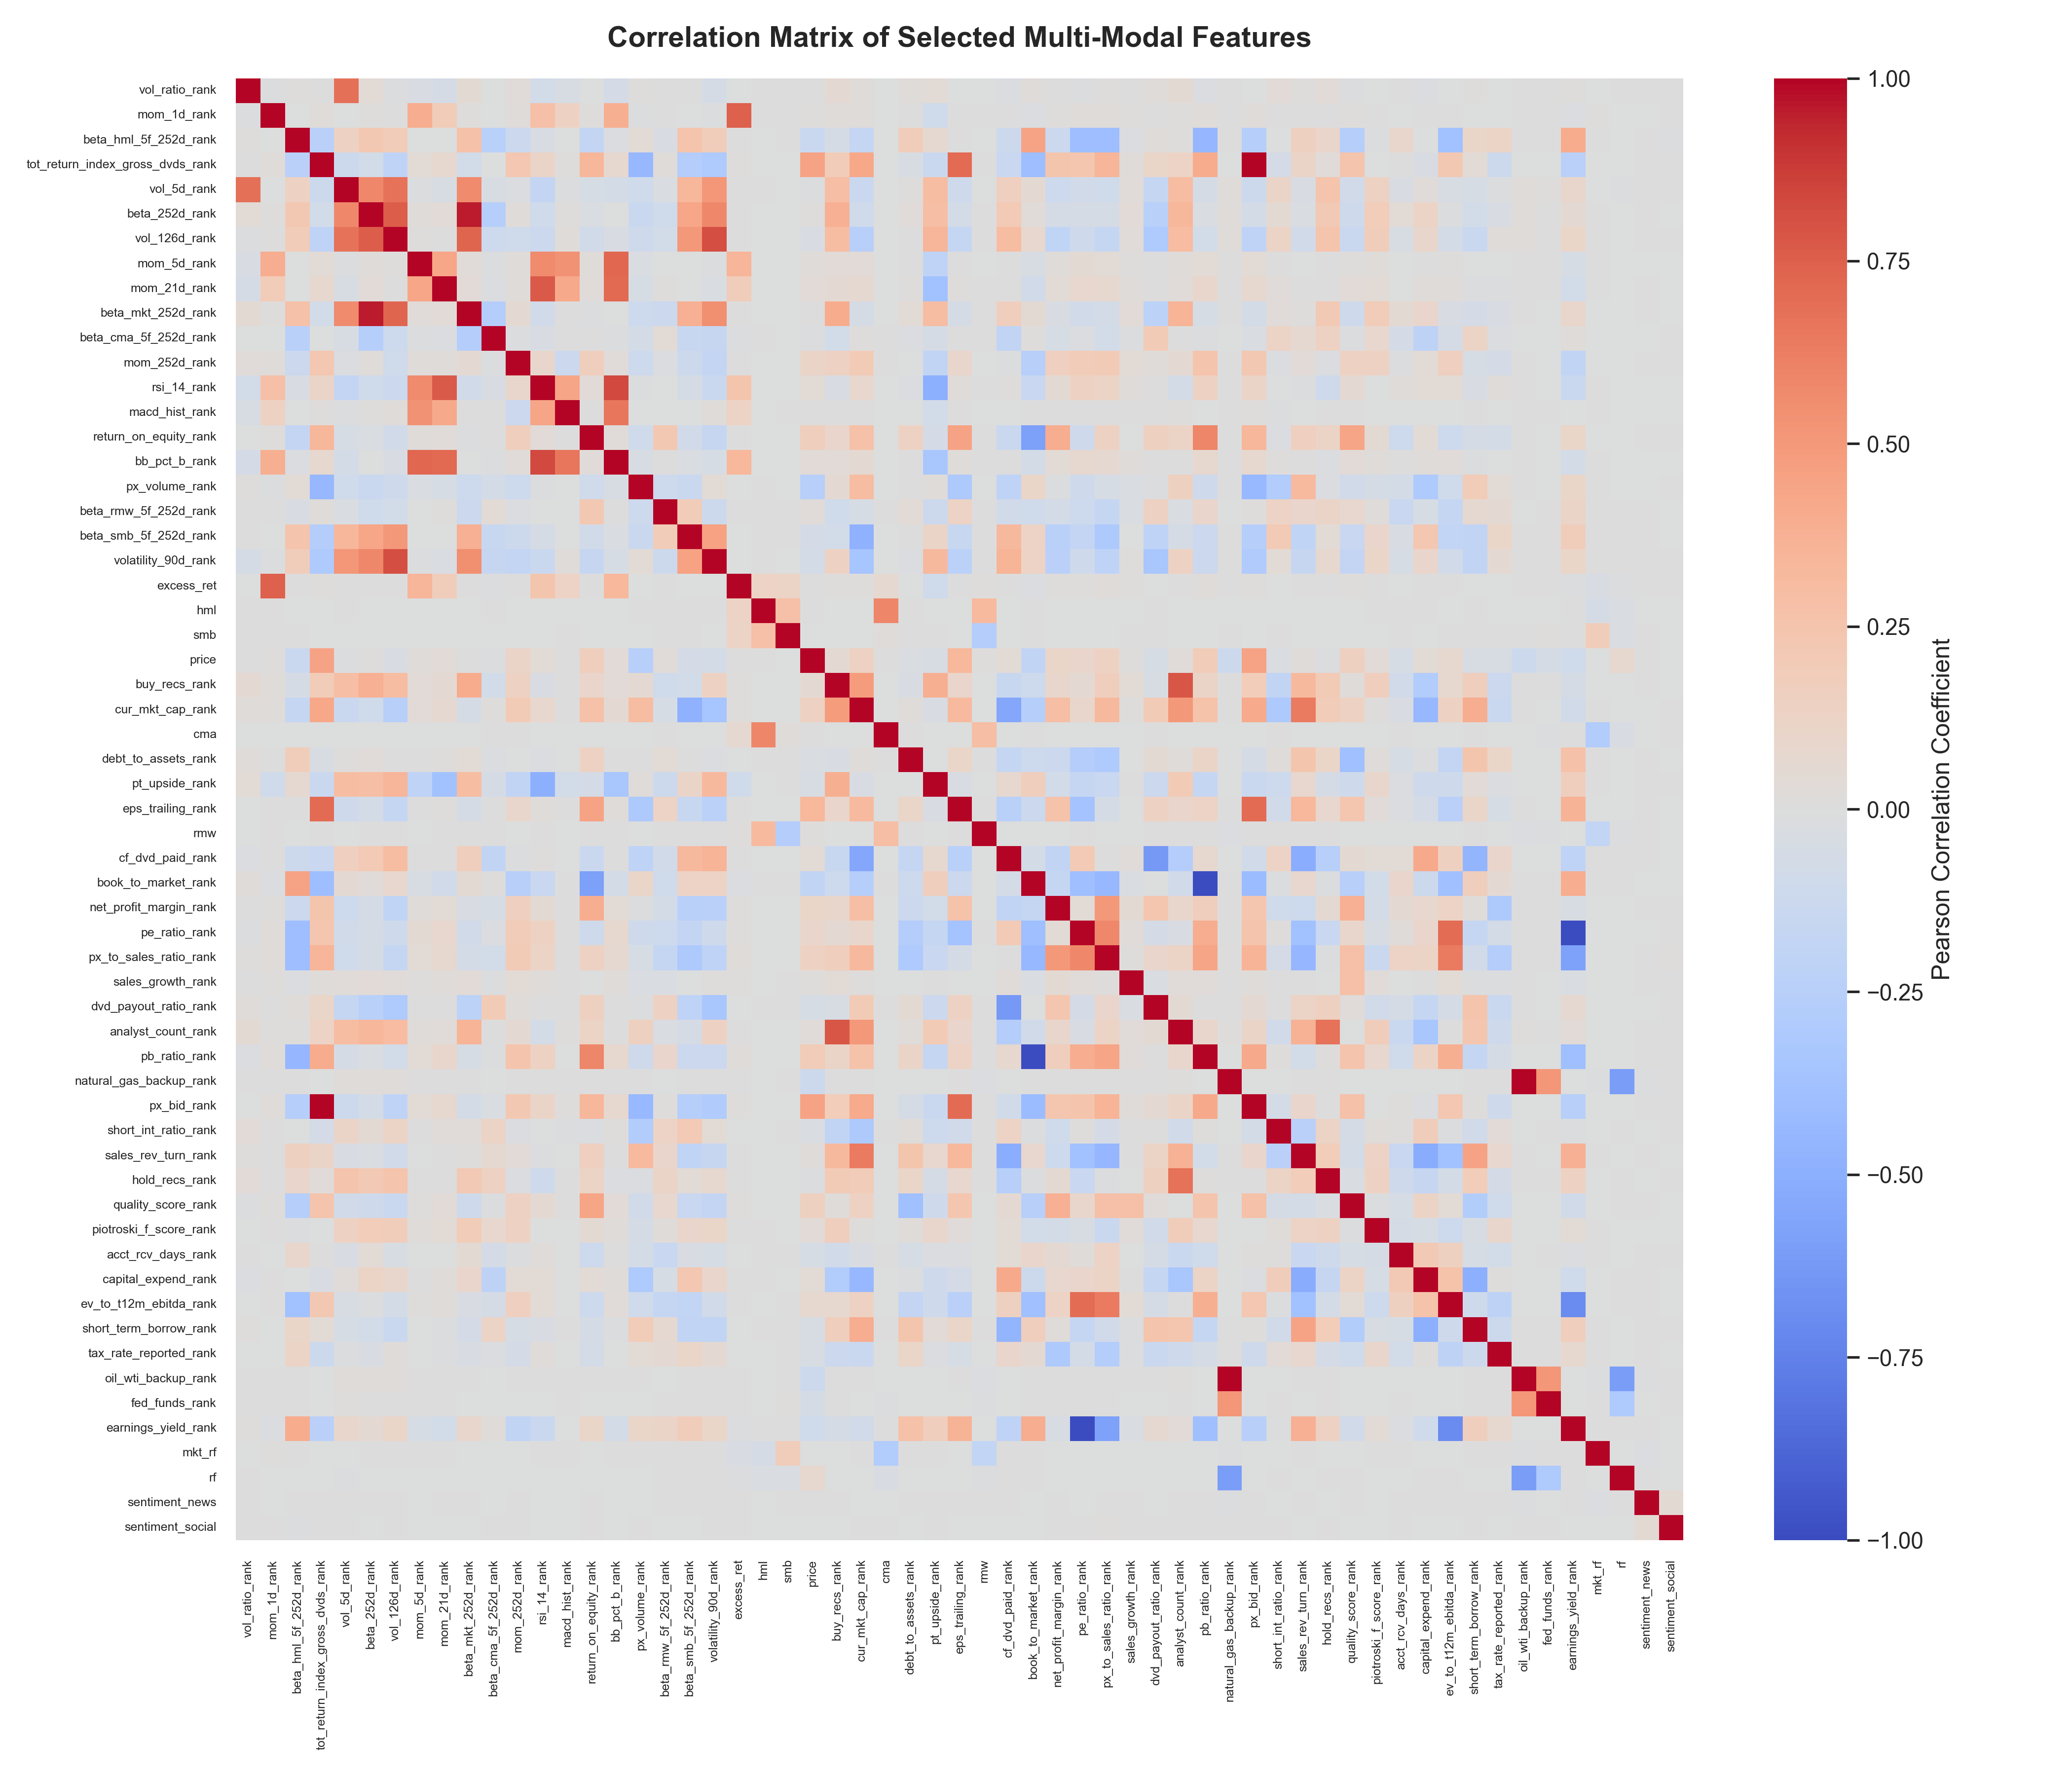
\includegraphics[width=0.82\textwidth]{./figures/selected_features_correlation.png}
\caption{Spearman Rank Correlation Heatmap of Selected 53 ML Features}
\label{fig:ch3_corr_heatmap}
\end{figure}

\begin{figure}[H]
\centering
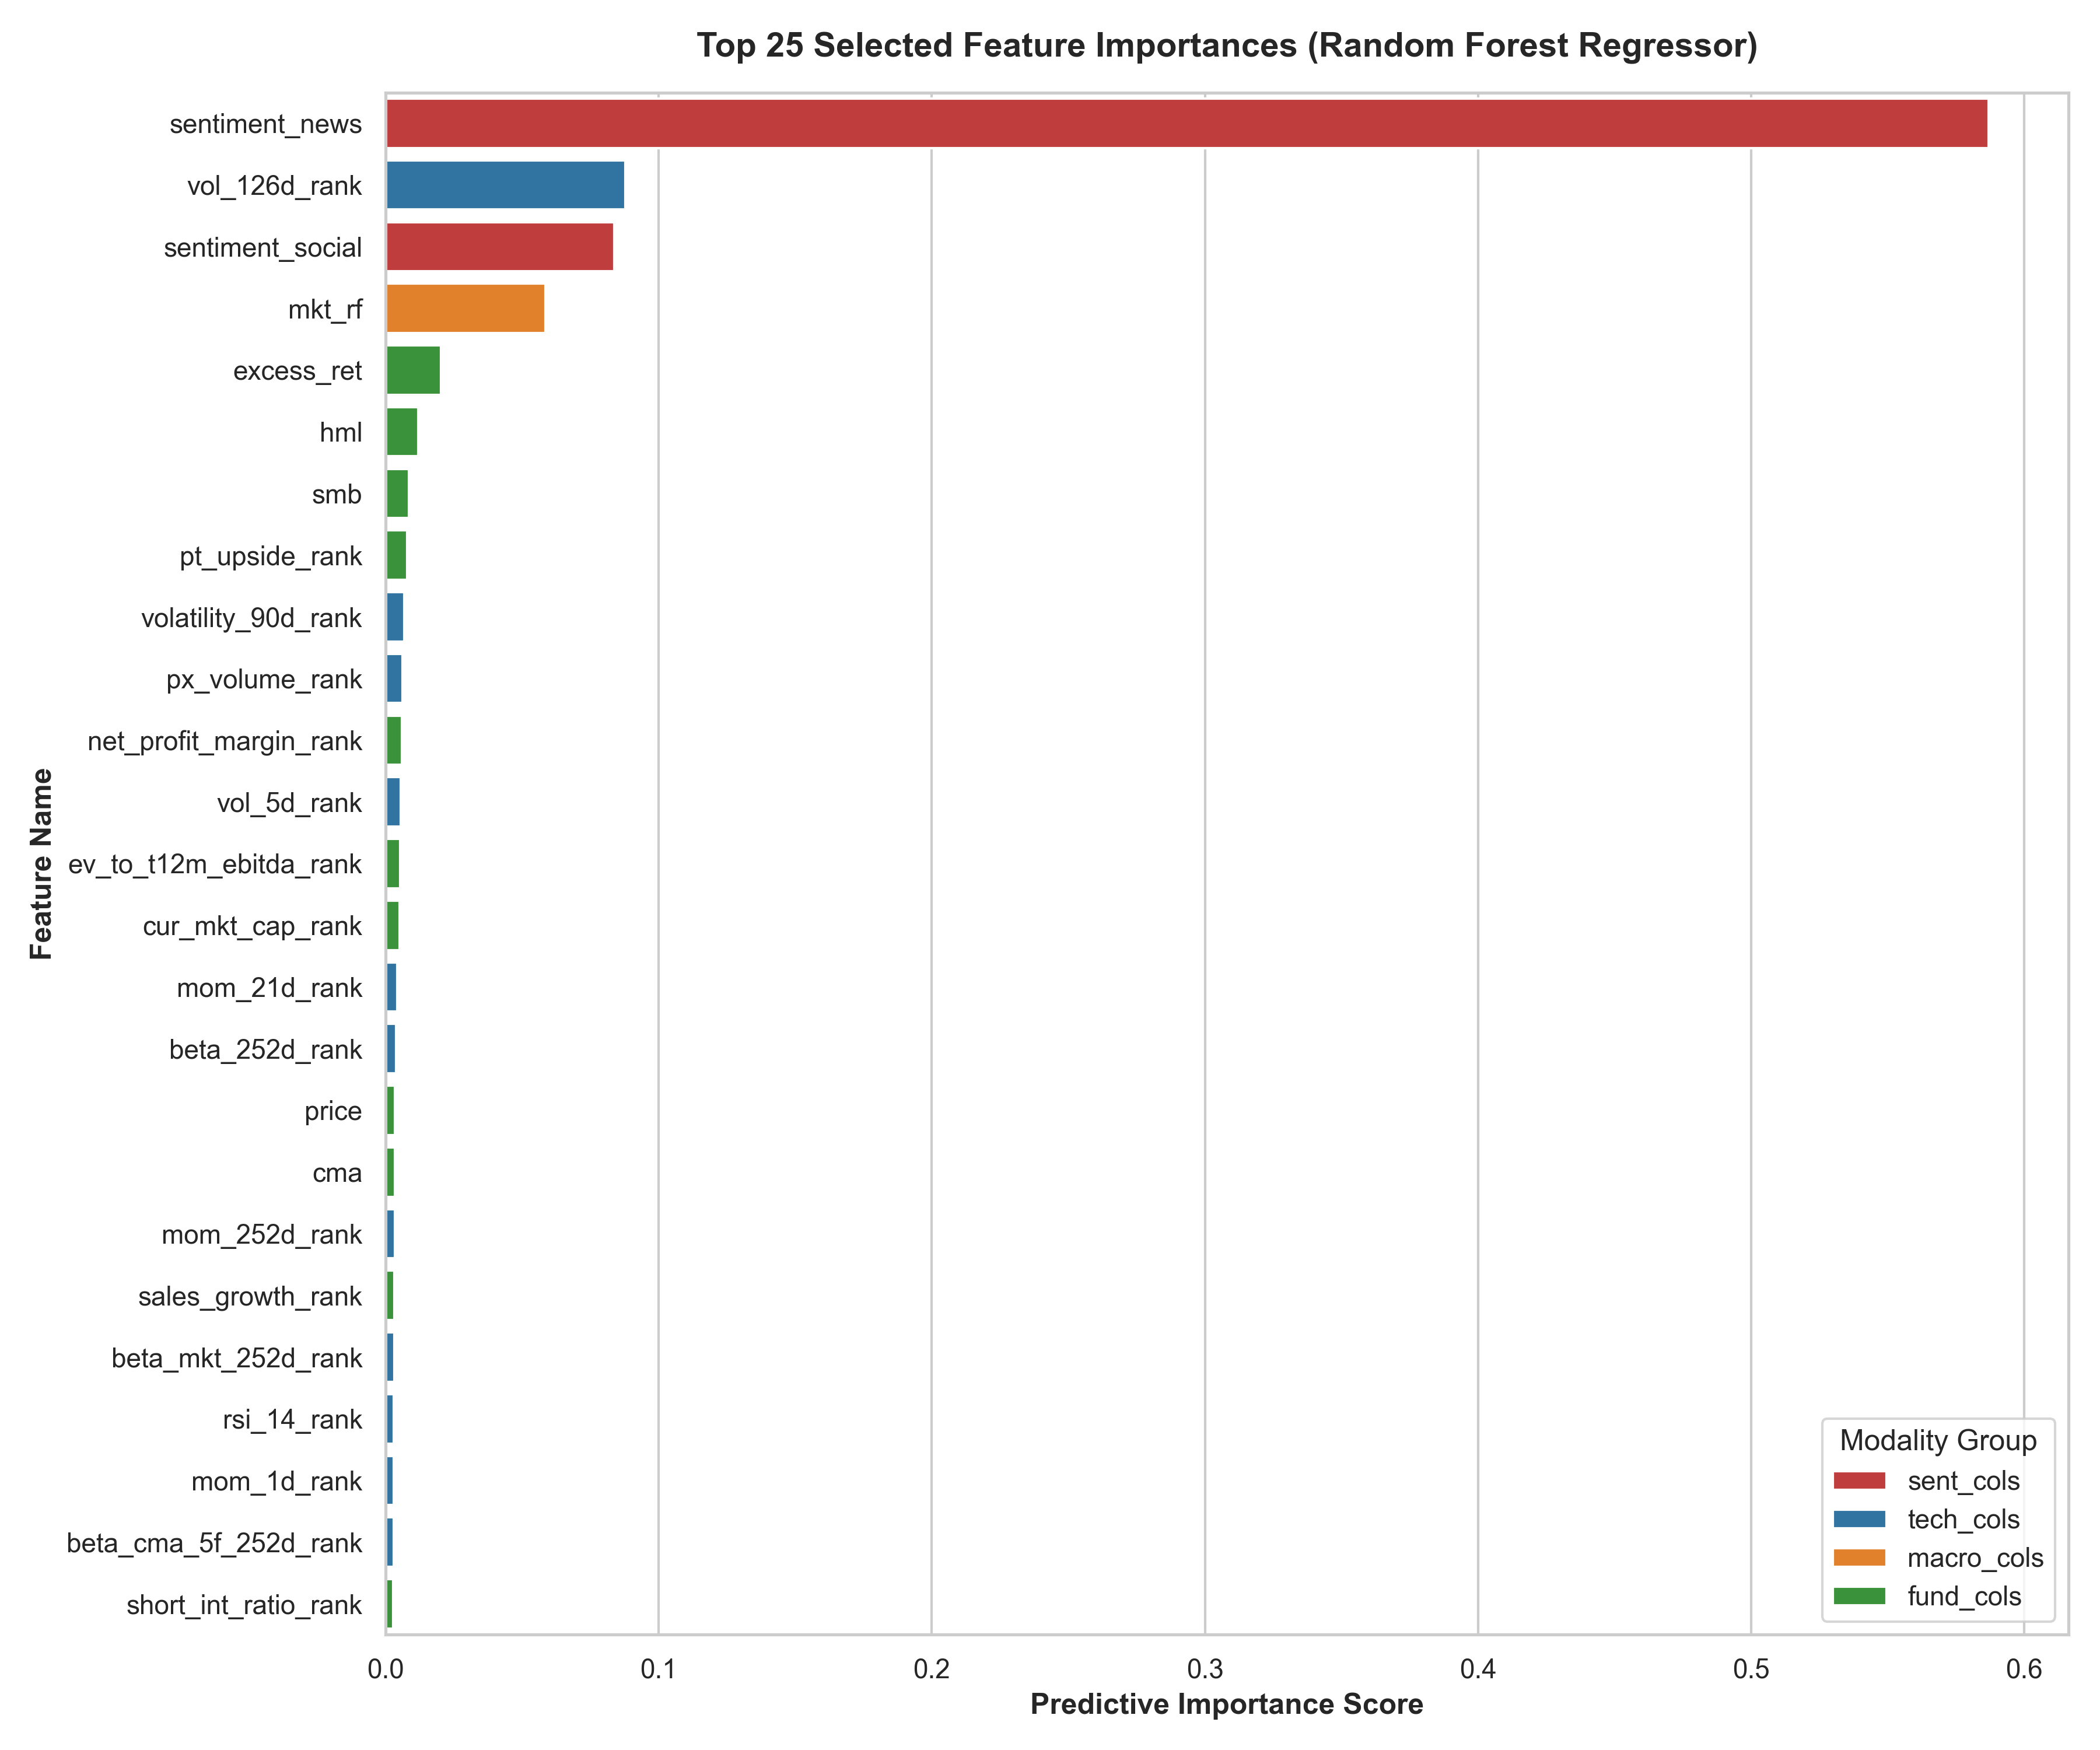
\includegraphics[width=0.82\textwidth]{./figures/selected_feature_importances.png}
\caption{Stage 3 Random Forest Feature Importance Rankings across Modalities}
\label{fig:ch3_rf_importance}
\end{figure}
